\chapter{Signal conditioning system design}
\section{System overview} \label{sec:system}
\begin{figure}
    \centering
    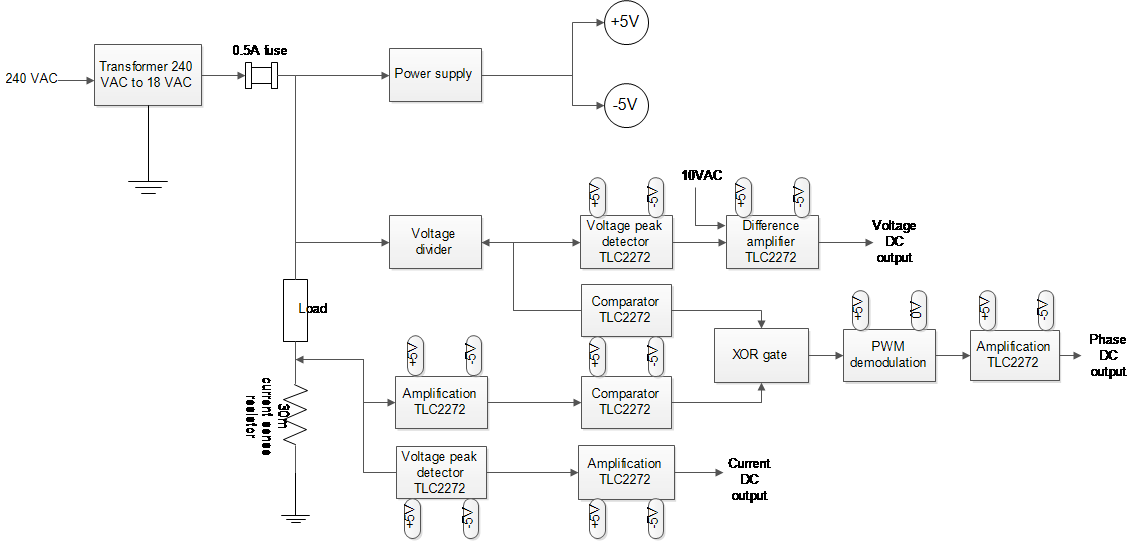
\includegraphics[width = 1\linewidth]{Figures/system_overview_2}
    \caption{System diagram}
    \label{fig:system_diagram}
\end{figure}

The TLC2272 rail-to-rail op amps were selected for all three transducers. This is due to their compact nature (2 op amps in one package as compared to the 1:1 ratio of the TL081), as well as their ability to produce output voltages much closer to the rails, which improves the resolution of the final values.
Each TLC2272 op amp draws approximately $2.4\SI{\milli}{\ampere}$\cite{TLC2272} from the $\pm5\si{\volt}$ supplies. As the system uses 8 op-amps, as well as an XOR gate, this amounts to a draw of approximately $\SI{20}{\milli\ampere}$. This is well within the specification they were designed for.









